\subsubsection{Navigation Stack}
\label{subsubsec:02navigatinStack}
Der Navigation Stack ist ein \"Uberbegriff f\"ur die Verbindung mehrerer Pakete. Aus den Odometrie- und Sensordaten wird eine Trajektorie zu einem vorher definierten Ziel geplant. Es werden Geschwindigkeits- und Lenkwinkeldaten ausgegeben, die den Roboter zu dem gegebenen Ziel f\"uhren.
\paragraph{Costmap}
F\"ur die Navigation wird eine Karte genutzt. Es wird unterschieden zwischen globaler und lokaler Costmap\footnote{http://wiki.ros.org/costmap\_2d}, zus\"atzlich liegen Informationen auf unterschiedlichen Schichten, sogenannten Layers.
\begin{itemize}
	\item Static Map Layer: diese Schicht beinhaltet Kartendaten aus bereits gemappten Umgebungen, falls vorhanden. Sie sind Teil der globalen Costmap und bleiben w\"ahrend der gesamten Laufzeit bestehen.
	\item Obstacle Map Layer: diese Schicht enh\"alt die Daten aus dem Laserscan, der mit dem Package \texttt{depthimage\_to\_laserscan} aus dem mit \texttt{pses\_kinect\_utilities} Median-gefilterten Tiefenbilder der Kinect2 Kamera erstellt wird. Hier werden also lokale Hindernisse gespeichert und bei Bedarf wieder entfernt. Diese Schicht ist Teil der lokalen Costmap.
	\item Inflation Layer: diese Schicht definiert einen Bereich um jedes erkannte Hindernis und \"uberlagert diesen mit einer Kostenfunktion (nah am Objekt hohe Bestrafung, weiter entfernt weniger Bestrafung). Die wichtigen Parameter sind \texttt{inflation\_radius} (\SI{1}{\meter}) und \texttt{cost\_scaling\_factor} (0.7 / 5). Diese Schicht ist ebenfalls Teil der lokalen Costmap. 
\end{itemize}

\paragraph{Globaler Planer} 
Anhang der Position des Roboters, der Costmap und des Zieles wird eine einfache Trajektorie geplant. Dabei wird weder die Dynamik des Rotobers betrachtet noch der Mindestabstand zu Hindernisse eingehalten. Es wurde mit dem navfn\footnote{http://wiki.ros.org/navfn} Planer gearbeitet.

\paragraph{Lokaler Planer}
Ausgehen von dem globalen Pfad wird ein lokaler Pfad geplant, der auf Hindernisse reagiert und die Ausma\ss{}e und Dynamik des Roboters bei der Planung mit in Betracht zieht. Es wurde sich f\"ur den TEB local planner\footnote{http://wiki.ros.org/teb\_local\_planner} entschieden, da er auch f\"ur nicht holonome Fahrzeuge gut geeignet ist. Die Qualit\"at der geplanten Trajektorie und des realen Fahrverhaltens wird ma\ss{}geblich von der Konfiguration der Parameter des Planers beeinflusst. Parameter mit sehr gro\ss{}em Einfluss sind in Tabelle \ref{tab:TEB} zusammengefasst.

\begin{table}[h]
	\centering
	\renewcommand{\arraystretch}{1.2}
	\begin{tabular}{p{4cm}l p{9cm}}
		Parameter & Wert  & Auswirkung \\ \hline
		dt\_ref & 0.5-0.75 & Besseres folgen der Trajektorie, weniger \"Uberschwingen (sehr wichtig)\\ 
		max\_vel\_x & 0.8 & Geschwindigkeitsbegrenzung vorw\"arts\\
		max\_vel\_x\_backwards & 0.5 & Geschwindigkeitsbegrenzung r\"uckw\"arts\\
		max\_vel\_y & 0.0 & Planer darf keine Geschwindigkeit in y-Richtung planen\\
		acc\_lim\_y & 0.0 & Planer darf nicht in y-Richtung beschleunigen\\
		max\_vel\_theta & 3.1 & Winkelgeschwindigkeit experimentell bestimmt f\"ur optimale Performance (gemessen ca. \SI[per-mode=fraction]{1.1}{\radian\per\second})\\
		acc\_lim\_x & 2 & x-Beschleunigung experimentell bestimmt f\"ur optimale Performance (gemessen ca. \SI[per-mode=fraction]{0.6}{\meter\per\second\squared})\\
		acc\_lim\_theta& 1.12 & Winkelbeschleunigung gemessen\\
		cmd\_angle\_instead\_ rotvel & True & Planer gibt Lenkwinkel und x-Geschwindigkeit aus (f\"ur nicht holonome Roboter) \\
		enable\_homotopy\_ class\_planning & False & Schnellere Planung, da nicht mehrere M\"oglichkeiten betrachtet werden
	\end{tabular}
	\caption{Parameter mit hohem Einfluss auf die Performance des TEB local planner.}
	\label{tab:TEB}
\end{table}

\paragraph{TF}
Jedes ver\"offentliche Topic wird mit einem Frame markiert. Um die Beziehung zwischen den dazugeh\"origen Koordinatensystemen herzustellen, kann das Package TF\footnote{http://wiki.ros.org/tf\#static\_transform\_publisher} genutzt werden. Darin wird jeweils zwischen zwei Systemen eine Beziehung definiert und somit ein TF-Baum erstellt. Eine Transformation definiert sich durch
\lstset{breaklines=true, basicstyle=\small}
\begin{lstlisting}
 <node pkg="tf" type="static_transform_publisher" name="Select_a_name" args="x y z qx qy qz qw PARENT CHILD 20" />.
\end{lstlisting}
Der Baum setzt sich, wie in Tabelle \ref{tab:TF} gezeigt, zusammen.
\begin{table}[h]
	\centering
	\renewcommand{\arraystretch}{1.2}
	\begin{tabular}{ll}
		Frame & Ursprung  \\ \hline
		map & map\_server \\
		odom & pses\_odometry \\
		base\_footprint & pses\_odometry \\
		base\_link & Navigation Stack \\
		base\_laser & Navigation Stack \\
		camera\_depth\_frame & LaserScan
	\end{tabular}
	\caption{TF-Baum mit dem Ursprung oben.}
	\label{tab:TF}
\end{table}

\paragraph{Debugging}
Beim Einrichten des Navigation Stack treten hin und wieder Probleme und Fehler auf. Die Korrektheit des TF-Baum l\"asst sich mit \texttt{rosrun rqt\_tf\_tree rqt\_tf\_tree} \"uberpr\"ufen. Die Informationen in einem Topic lassen sich mit \texttt{rostopic echo TOPIC} auslesen und Publisher sowie Subscriber mit \texttt{rostopic info TOPIC} ausgeben. Die Verbindungen zwischen laufenden Nodes wird mit \texttt{rosrun rqt\_graph rqt\_graph} dargestellt.\\
Sobald die grundlegende Struktur funktioniert, hilft das grafische Programm RViz\footnote{http://wiki.ros.org/rviz} weiter. Ob die Transformationen zwischen den Koordinatensystemen korrekt sind l\"asst sich damit \"uberpr\"ufen. Au\ss{}erdem l\"asst sich damit die globale Karte, Costmap und der Laserscan darstellen und auf Korrektheit pr\"ufen. Zus\"atzlich ist die Position und der Footprint (digitale Repr\"asentation des Fahrzeugs) visualisierbar, welcher sich beim Fahren auch verschieben. Dabei sollte beachtet werden, dass sich die dargestellte Position des Fahrzeugs nur verschiebt, wenn der Motor angesteuert wird, beim Drehen des Hallsensors ohne Ansteuerung wird vom \texttt{pses\_odometrie} Package keine Positions\"anderung gepublisht. Sobald die Karte und Position des Fahrzeugs korrekt wiedergegeben werden, ist es sinnvoll in RViz \"uber den Button \texttt{2D Nav Goal} ein Ziel zu setzen und die geplante Trajektorie ausgeben zu lassen.\\
Es sei angemerkt, dass ein positiver Wert f\"ur die Stellgr\"o\ss{}e des Lenkwinkels einen Einschlag nach rechts bedeutet, der TEB local planner allerdings mit positiven Werten einen Lenkeinschlag nach links meint.

\paragraph{Hilfreiche Tools}
F\"ur Testfahren ist es hilfreich das Fahrzeug und einen Laptop mit dem selben WLAN-Netzwerk zu verbinden und per SSH auf das System des Fahrzeugs zuzugreifen. Dazu wird die IP-Adresse des Fahrzeugs ben\"otigt (\texttt{ifconfig}) und die Verbindung vom Laptop zum Fahrzeug geschieht dann \"uber \texttt{ssh user@IP}. Daf\"ur ist es ratsam einen WLAN-Hotspot, beispielsweise \"uber ein Handy, einzurichten.\\
Mit dem Tool \texttt{dynamic\_reconfigure}\footnote{http://wiki.ros.org/dynamic\_reconfigure} lassen sich Parameter w\"ahrend der Laufzeit ver\"andern. Wurde der Knoten entsprechend konfiguriert, wird der Parameter auf der per SSH verbundenen Konsole mit \texttt{rosrun dynamic\_reconfigure dynparam set NODE PARAMETER VALUE} ge\"andert. Somit kann w\"ahrend einer Testfahrt an der Performance des Fahrzeugs gearbeitet werden, ohne an den Arbeitsplatz zur\"uckkehren zu m\"ussen.\\
Eine weitere M\"oglichkeit zur Kontrolle \"uber das Netzwerk bietet die Konfiguration verteilter Systeme\footnote{http://wiki.ros.org/ROS/Tutorials/MultipleMachines}. Da ROS ohnehin \"uber Netzwerkstandards kommuniziert, bietet es die Option Topics im Netzwerk zu verteilen. Das bedeutet, dass die Nodes auf dem Fahrzeug gestartet und die Topics auf einem Laptop, der im selben Netzwerk h\"angt, durch RViz visualisiert werden k\"onnen. Dadurch kann w\"ahrend einer Testfahrt mit dem Navigation Stack die Karte und Trajektorie kontrolliert werden. Zudem ist es m\"oglich Ziele zu setzen und die aktuelle Position des Fahrzeugs vorzugeben. Dies geschieht \"uber den Button \texttt{2D Pose Estimate} und dient dazu den Roboter in der Karte zu positionieren. Die Konfiguration auf dem Fahrzeug, sowie auf dem Laptop folgt diesem Schema:
\begin{lstlisting}
Auf Fahrzeug: 
IP herausfinden (ifconfig) 
In jedem Terminal, in dem ein Topic am Laptop braucht wird:  
  export ROS_IP=machine_ip_addr <- IP des Fahrzeugs 
  node/launch-file starten

Auf Laptop: 
Terminal: 
  export ROS_MASTER_URI=http://172.  .  .  :11311 <- IP Fahrzeug
  IP herausfinden (ifconfig) 
  export ROS_IP=machine_ip_addr (Laptop IP) 
  rviz
\end{lstlisting}

\paragraph{Freier Rundkurs und Hindernisparcours}
Die beiden Aufgaben Rundkurs ohne sowie mit Hindernissen sind vom Grundprinzip sehr \"ahnlich und werden beide mit dem Navigation Stack bew\"altigt. Die Planung des zu fahrenden Pfades bleibt gleich, nur einige Parameter f\"ur die Fahrt machen einen Unterschied f\"ur die beiden Aufgaben. Die Dateien zum Starten und Konfigurieren des Navigation Stack befinden sich in Anhang \ref{subsec:appendixNS}. Die sich f\"ur den freien Rundkurs und Hindernisparcours unterscheidenden Parameter sind jeweils mit dem Kommentar \texttt{for obstacle parcour} vermerkt.

\begin{figure}[h]
	\centering
	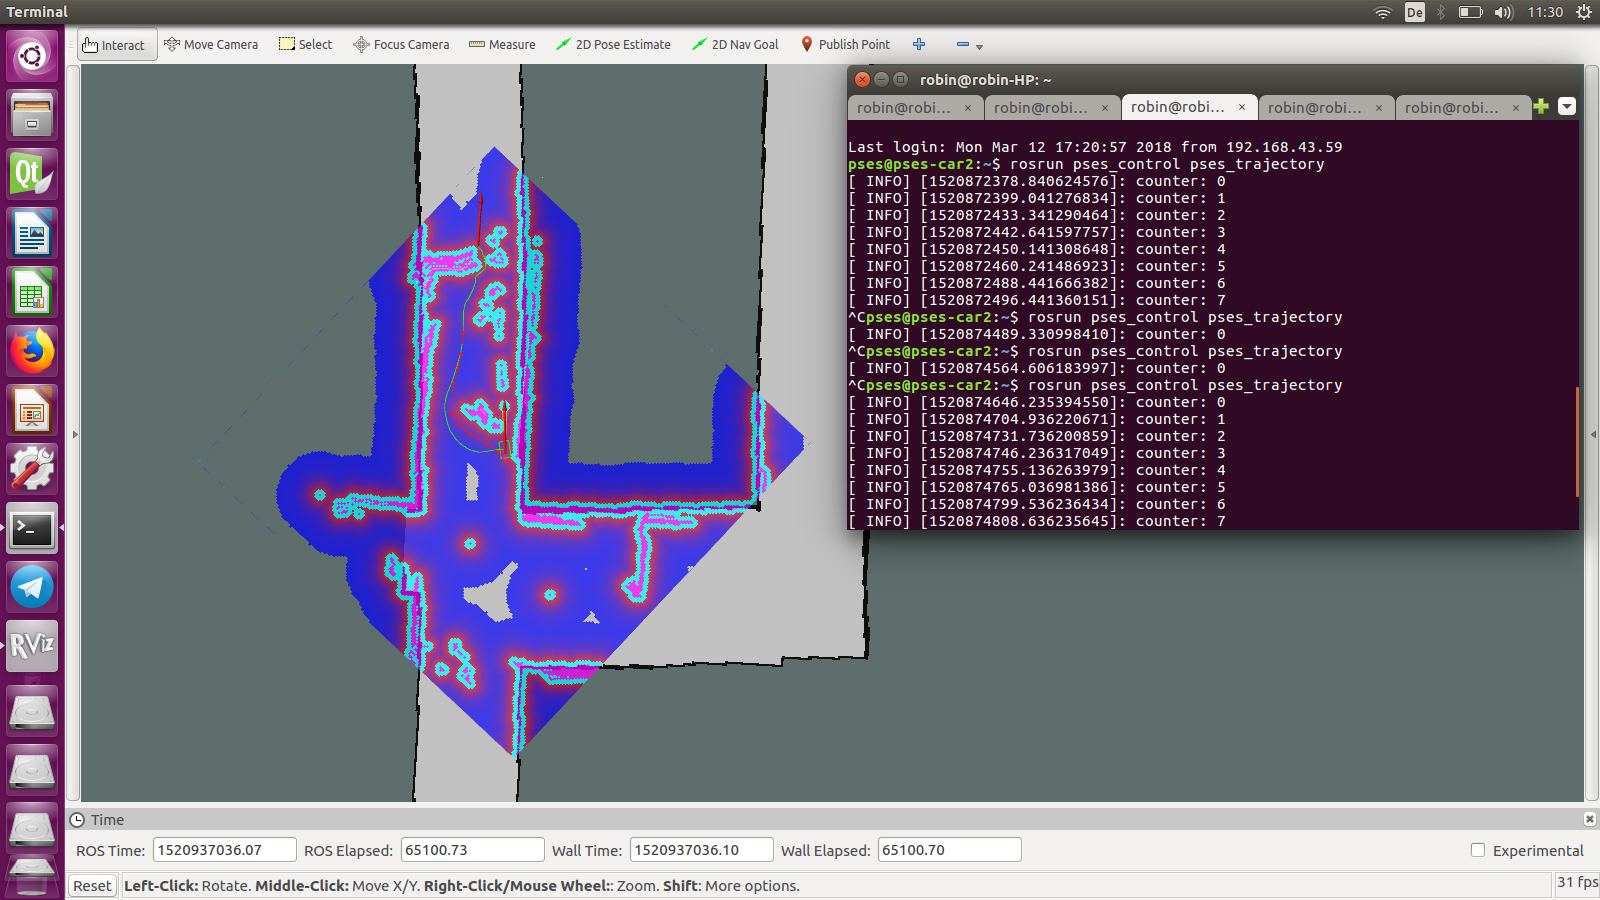
\includegraphics[width=0.8\textwidth,trim=2.4cm 0cm 0cm 1cm,clip]{pics/rviz.png}
	\caption{Ausschnitt aus RViz mit der Costmap, dem Footprint des Fahrzeugs und der Zielf\"uhrung sowie das Terminal, in dem der Fahrknoten gestartet ist.}
	\label{fig:rviz}
\end{figure}